\section{Low Threshold Cherenkov Counter}

\subsection{Geometry}
The LTCC mirror geometry is implemented through the native GEMC geometry API. The elliptical mirrors are made through a subtraction of
two G4Ellipsoid. The hyperbolic mirror are built using Geant4 polycone approximating the mathematical shape using about 30 segments.
The cylindrical mirrors are made of G4Tubs.

The LTCC Winston cones are of three types: small, medium and large. Three CAD models are tessellated and imported in the simulation, and
then are copied into 36 WC / sectors using the perl api.

Finally, the LTCC Box, mirror support structure and additional support hardware are imported directly from the engineering CAD models.
The \F{ltccGeometry} shows details of the geometry implementation.

\begin{figure}
	\centering
	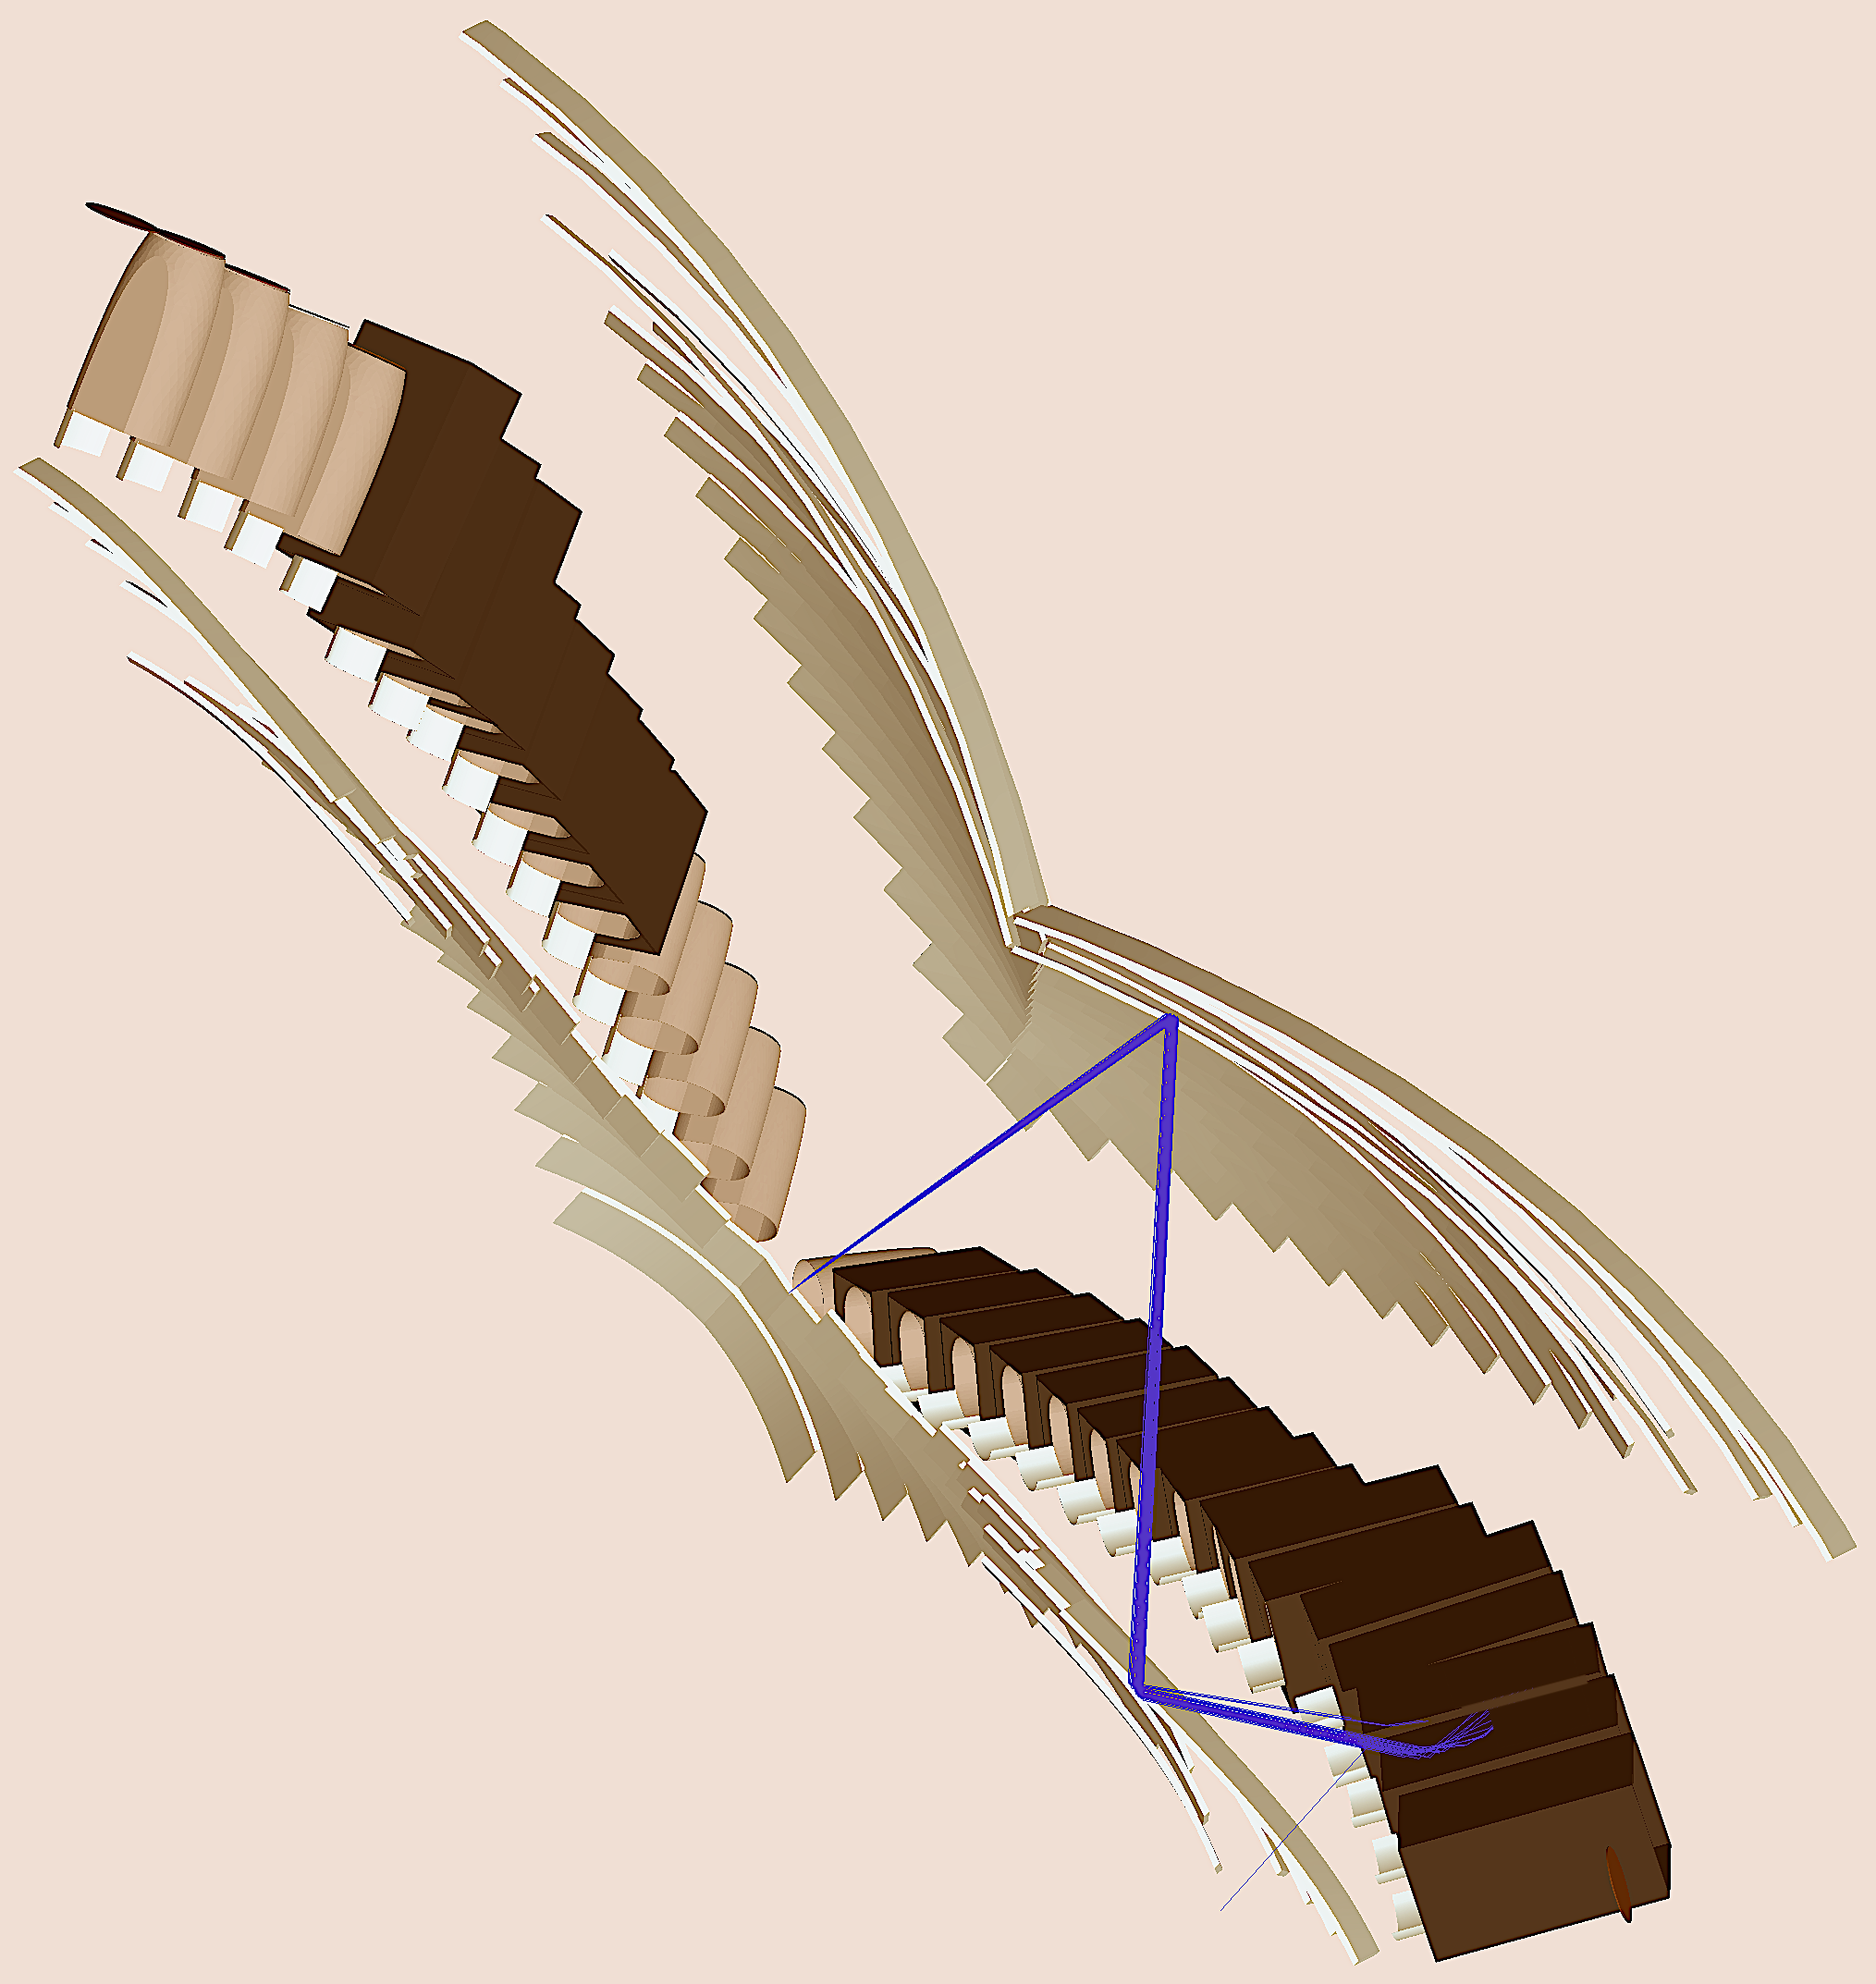
\includegraphics[width=0.95\columnwidth,keepaspectratio]{img/ltccGeometry.png}
	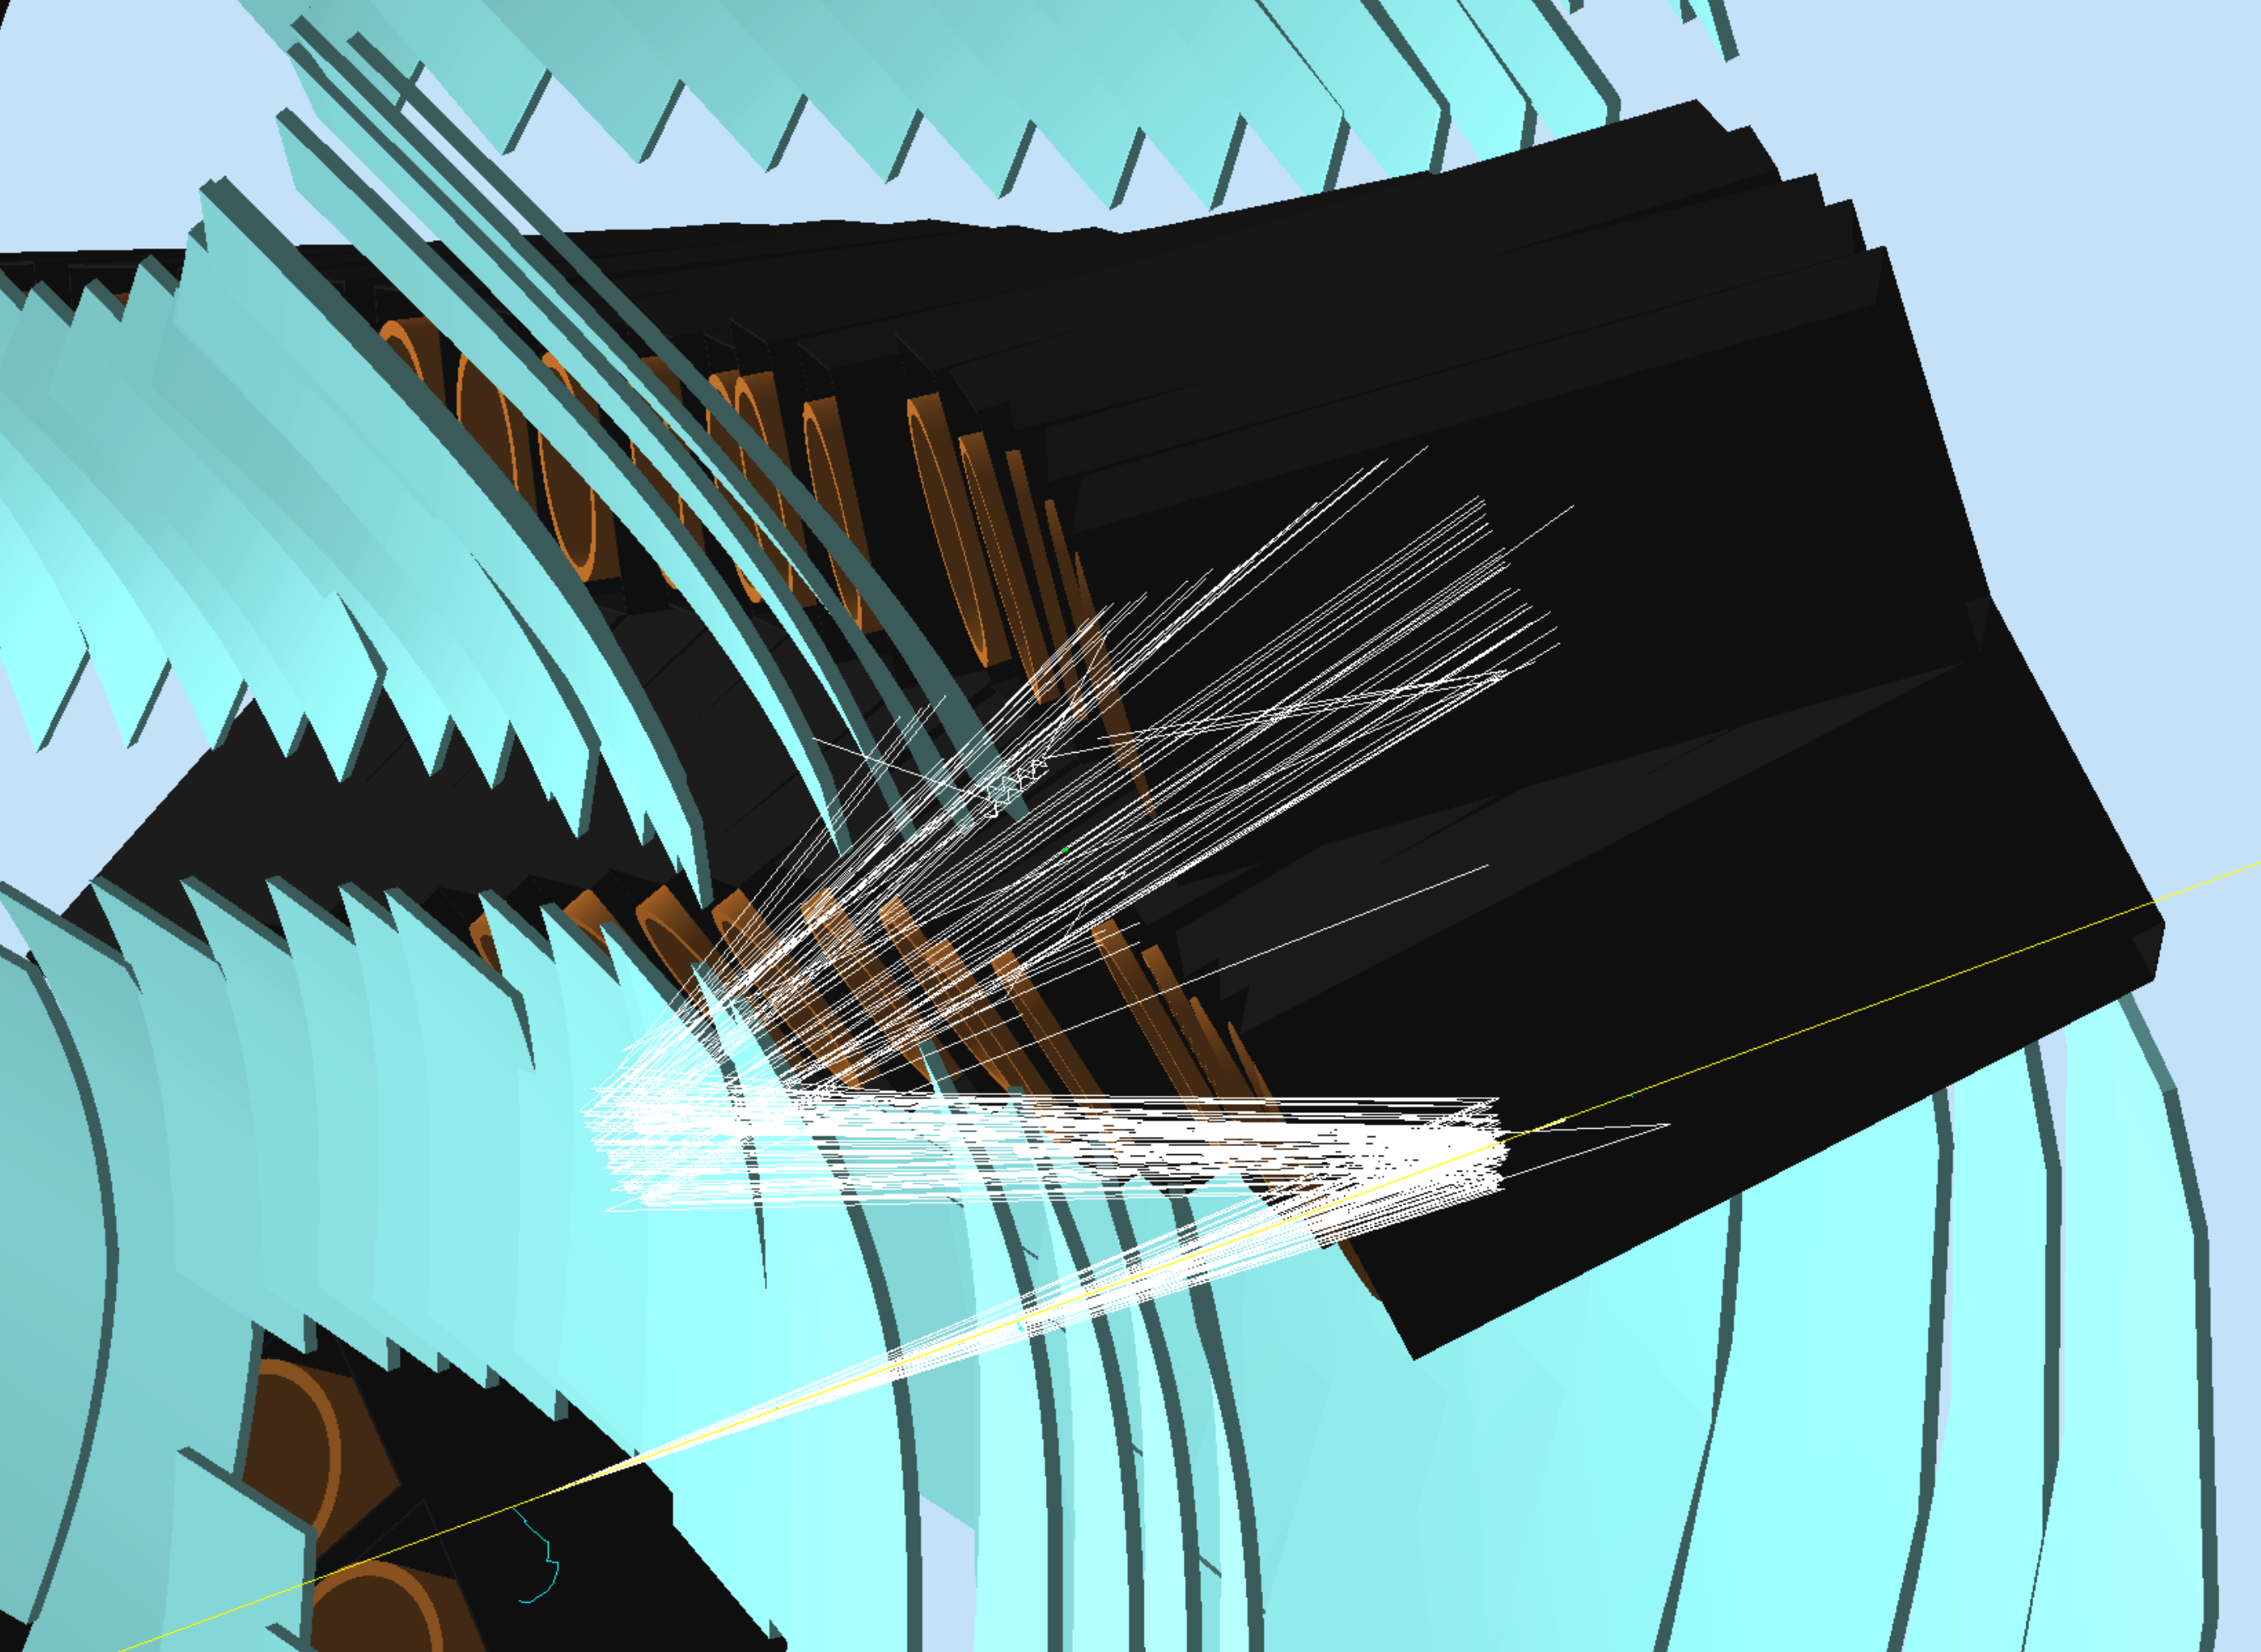
\includegraphics[width=0.95\columnwidth,keepaspectratio]{img/ltccDetail.png}
	\caption{Top: a 6 GeV pion passing through the TCC gas volume and emitting Cherenkov photons. The light cone
            bounces from the elliptical to the hyperbolic to the Winston cone and finally reaches the PMT. The
            frame of the LTCC, imported from the CAD engineering model, is visible.
            Bottom: details of the light path through the mirrors. }
	\label{fig:ltccGeometry}
\end{figure}

The refractive index of the $C_4F_10$ and its transparency is included in the material optical properties and taken
into account during the Geant4 transportation of the photons.

The mirror and Winston cones reflectivity is associated with the mirror optical properties and are taken into
account and taken into account during the Geant4 transportation of the photons.

The quartz window PMT quantum efficiency are associated with the PMT face optical properties and are taken into account in
the digitization routine.

\subsubsection{Geometry Location on GitHub}
The Github location of the GEMC perl API script is  \url{https://github.com/gemc/detectors/tree/master/clas12/ltcc}.


\subsection{Digitization}

Photons that impinged on the PMT faces are processed with the digitization routine.
For each photon collected undergoes the quantum efficiency algorithm at its wavelength to decided if it's finally detected.
The ADC is calculated and smeared using the single photo-electron peak position and sigma from the calibration database.


\subsubsection{Timing}

The time average of all the photons is saved in the output.

\subsubsection{Summary of CCDB Table Used}

\begin{itemize}
	\item /calibration/ltcc/spe
\end{itemize}

\subsection{Digitized Bank}

The digitized output bank has $ID=1400$, and the variables are summarized in Table \ref{tab:ltccBank}.

\begin{table}[h]
	\begin{center}
		\begin{tabular}{| c | c | c |}
			\hline \hline
			Variable    & Description                                        & Tag  \\
			\hline
             sector  &                                     clas12 sector  &    1 \\
               side  &                               left or right index  &    2 \\
            segment  &                                           segment  &    3 \\
                ADC  &                                               ADC  &    4 \\
               time  &                           average time of the hit  &    5 \\
               nphe  &                  number of photoelectrons arrived  &    6 \\
              npheD  &                 number of photoelectrons detected  &    7 \\
               hitn  &                                        hit number  &   99 \\
			\hline \hline
		\end{tabular}
	\end{center}
	\caption{The digitized LTCC bank.}\label{tab:ltccBank}
\end{table}

\subsubsection{Time Window}
The time window  of the LTCC is set to 5 ns.

\subsubsection{Process Routine Git Repository Location}
The LTCC hit process routine location in git is \url{https://github.com/gemc/source/blob/master/hitprocess/clas12/ltcc_hitprocess.cc}
